\chapter{Theory}
\section{Terahertz radiation}
This thesis will show the means of generating Terahertz ($\si{\tera\hertz}$) radiation, with two non-linear crystals.
As the name describes, its frequency regime lies at about $(0.3-30)\cdot10^{12}\,\si{\hertz}$.
Its wavelength can be easily calculated by
\begin{equation}
    \lambda = \frac{c}{\nu}
\end{equation}
with the speed of light $c$ and its frequency $\nu$.
Which results in a wavelength of about $\SI{100}{\micro\meter}-\SI{1}{\milli\meter}$.
This means it lies between infrared and microwave radiation.
$\si{\tera\hertz}$ radiation is caused by various non-linear effects which only occur at relatively high intensities.
The need for high intensities, as well as the lack of emitters, makes it hard to generate it efficiently.
The result is the so-called $\si{\tera\hertz}$ gap that is slowly being closed by new techniques and advances in science.
Some of these are the generation of $\si{\tera\hertz}$ radiation through in- and inorganic crystals, as well as the use of semiconductors.
\\
$\si{\tera\hertz}$ radiation is non-ionizing but is absorbed by water.
This makes it of particular interest for medical uses.
The water absorption will be shown later. 
%%%%%%%%%%%%%%%%%%%%%%%%%%%%%%%%%%%%%%%%%%%%%%%%%%%%%%%%%%%%%%%%%%%%%%%%%%%%%%%%%%


%%%%%%%%%%%%%%%%%%%%%%%%%%%%%%%%%%%%%%%%%%%%%%%%%%%%%%%%%%%%%%%%%%%%%%%%%%%%%%%%%%
\section{Non-linear crystals}
Optical non-linear crystals exhibit a non-linearity in their second-order susceptibility $\chi_2$ or in even higher orders.
For this, they show special non-linear effects at high electric field strengths.
For different purposes, different kinds of crystals are in use.
\subsection{Zinc telluride}
\label{sec:znte}
One of the crystals that is in use to generate $\si{\tera\hertz}$ radiation is zinc telluride (ZnTe). 
It allows the generation of a wideband coherent $\si{\tera\hertz}$ field through means of optical rectification \cite{ZnTe_Nahata_Weling_1996}, which is described in section \ref{sec:optic_ref}.
It should be mentioned that ZnTe has a phonon resonance at $\SI{5.3}{\tera\hertz}$ which limits the bandwidth of emitted radiation and its ability to detect radiation of that or higher frequencies \cite{phonon_modes}.
Because optical rectification is a non-linear effect, it is important to align the laser to the $(110)$ axis of the crystal.
The angle between the $(001)$ direction and the polarization of the pump beam is also important.
It can be seen in figure \ref{fig:polarization_dependence_angle} that two angles give the strongest signal.
\begin{figure}
    \centering
    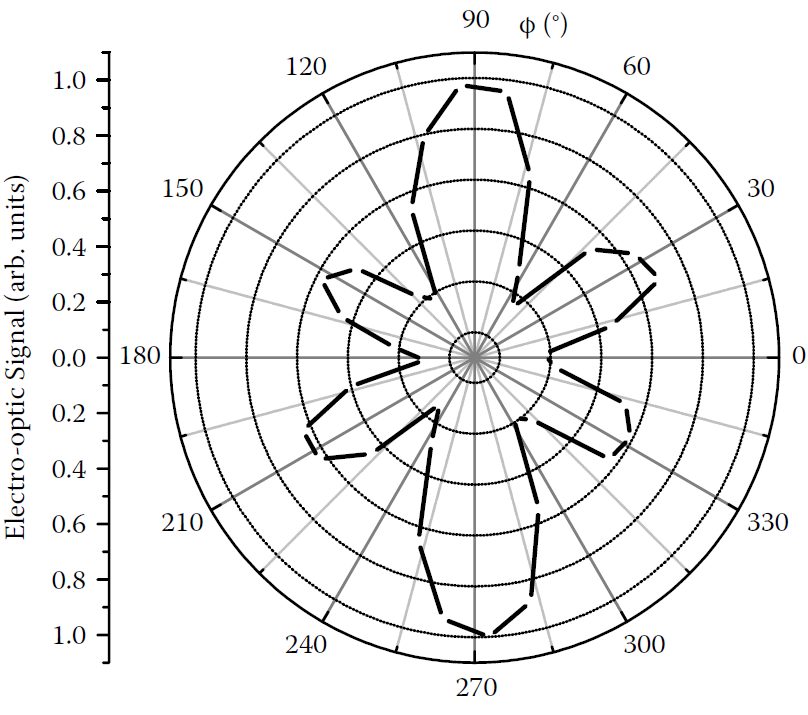
\includegraphics[width=0.4\textwidth]{refferenced_pic/degreedepenceZnTe.png}
    \caption{The plot shows the angle-dependent emission of $\si{\tera\hertz}$ radiation in ZnTe.
    The angle is between the $(001)$ direction of the crystal and the polarization of the pump beam. An angle of $\theta = \SI{90}{\degree}$ however relates to the pump beam polarization being parallel to the $(001)$ axis.
    The plot is taken from source \cite{selig}.}
    \label{fig:polarization_dependence_angle}
\end{figure}
It is also used as a detection crystal for the $\si{\tera\hertz}$ field.
The ZnTe changes the polarization of the incoming probe beam dependent on the field strength of the $\si{\tera\hertz}$ radiation.
This effect is discussed in section \ref{sec:eos}.
The refractive index of ZnTe at $\SI{800}{\nano\meter}$ is $n_\text{ZnTe} = 2.85$.

\textbf{Platzhalter für Bild von ZnTe struktur}

\subsection{Gallium phosphide}
The other crystal that is used to generate $\si{\tera\hertz}$ radiation is gallium phosphide (GaP).
It is a common emitter of $\si{\tera\hertz}$ radiation with a broad spectrum.
This crystal also exhibits a phonon resonance, but at a much higher frequency of about $\SI{11}{\tera\hertz}$ \cite{wiki_book}.
As well as ZnTe, GaP needs to be stimulated by the laser along its $(110)$ axis.
The refractive index of GaP at $\SI{800}{\nano\meter}$ is $n_\text{GaP} = 3.193$.

\textbf{Platzhalter für Bild von GaP struktur}
%%%%%%%%%%%%%%%%%%%%%%%%%%%%%%%%%%%%%%%%%%%%%%%%%%%%%%%%%%%%%%%%%%%%%%%%%%%%%%%%%%


%%%%%%%%%%%%%%%%%%%%%%%%%%%%%%%%%%%%%%%%%%%%%%%%%%%%%%%%%%%%%%%%%%%%%%%%%%%%%%%%%%
\section{Optical rectification}\label{sec:optic_ref}
To produce $\si{\tera\hertz}$ radiation advantage is taken from optical rectification or rather a kind of difference frequency mixing that is very similar to optical rectification.
Optical rectification is a second-order non-linear effect and thus can be just observed in non-linear materials.
This effect causes a DC polarization in the crystal.
If the DC polarization is moduled correctly it will cause $\si{\tera\hertz}$ radiation.
The DC polarization occurs when an outer electric field interacts with the crystal.
Because of the non-linear structure and in turn the anharmonic potential of crystal charges, the charges oscillate further in one direction than the other.
The displacement of charge is what causes the DC polarization.
To discuss the effect in detail the effect of the electric field on the polarization needs to be looked at.
Polarization is defined as

\begin{equation}
P = \chi(E) E \epsilon_0
\end{equation}

and is directly proportional to the electric field $E$ and the susceptibility $\chi(E)$.
Which in turn can be expanded to 

\begin{equation}
    \chi(E) = \chi_0 + \chi_1 E +\chi_2 E^2 + ...   \, .
\end{equation}

As described earlier, optical rectification is a second-order effect and is described by the $P_\text{nl} = \chi_2 E^2$ term.
Because the laser produces electromagnetic radiation at the whole bandwidth of frequencies $\omega + \symup{\Delta}\Omega$, in a gaussian profile, it is necessary to consider all of those electric fields mixing inside the crystal.
To simplify it is best to look at just two electric fields.
One of those electric fields oscillates at frequency $\omega_\text{i}$ and the other at frequency $\omega_\text{j}$.
The resulting second-order polarization term 

\begin{equation}
    P_\text{nl} = \chi_2 \epsilon_0 \frac{E_0^2}{2}\left[\cos((\omega_\text{i} - \omega_\text{j})t) + \cos((\omega_\text{i} + \omega_\text{j})t)\right]
\label{eq:two_freq_mixing}
\end{equation}

shows a \textbf{cosine} with a difference dependency $\omega_\text{i}-\omega_\text{j}$ and one with a sum dependency $\omega_\text{i}+\omega_\text{j}$.
The one with the difference dependency results in the generation of $\si{\tera\hertz}$ radiation. % the one with the sum depends is important for second harmonic generation
The sum term of equation \eqref{eq:two_freq_mixing} is not important for $\si{\tera\hertz}$ generation and will be neglected in further calculations \cite{wiki_book}.
If the whole bandwidth $\omega + \symup{\Delta}\Omega$ is now taken into account all the frequencies interact with the crystal.
This results in a polarization dependency on the bandwidth $\symup{\Delta}\Omega$ as such
\begin{equation}
    P_{\symup{\Delta}\Omega} = \chi_2 \epsilon_0 \frac{E_0^2}{2}\cos(\symup{\Delta}\Omega t) \, ,
    \label{eq:polarization_depens}
\end{equation}
where $\epsilon_0$ is the vacuum permittivity.
With a bandwidth in the femtosecond regime, the resulting change in polarization generates $\si{\tera\hertz}$ radiation \cite{book_optical_rectification}\cite{wiki_book}.
\\\\
% Because the change in polarization is also dependent on the pump beam electric field, as seen in equation \ref{eq:polarization_depens}, part of the experiment is to change the pump fluence.
% The fluence is defined as 
% \begin{equation}
%     H = \int_{0}^{t} E_\text{irr} \symup{d}t
%     \label{eq:fluence}
% \end{equation}
% with $E_\text{irr}$ being the irradiance.
% The irradiance 
% \begin{equation}
%     E_\text{irr} = \frac{\Phi}{A}
%     \label{eq:irradiance}
% \end{equation} 
% is defined as the radiant flux $\Phi$ per area $A$.
% \\\\
The process of $\si{\tera\hertz}$ generation can also be explained by the excitation of higher energy levels.
It is visualized in figure \ref{fig:freq_mix}.
\begin{figure}
    \centering
    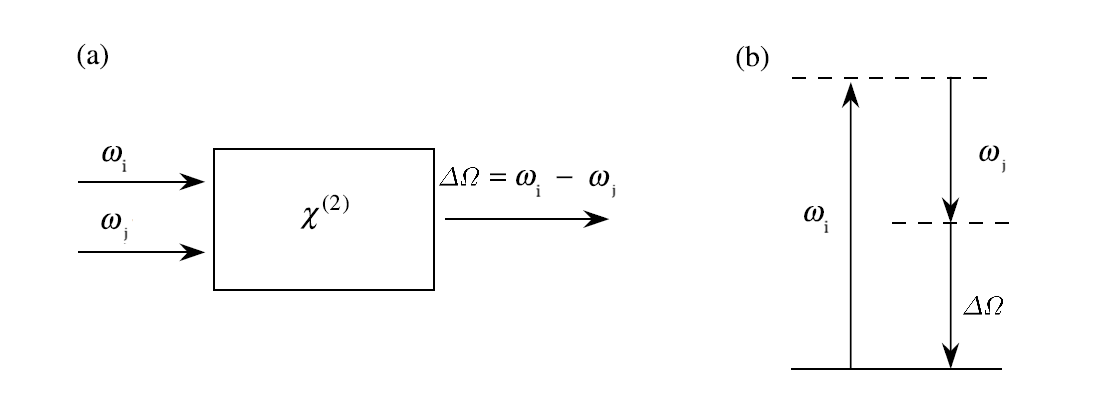
\includegraphics[width=\textwidth]{refferenced_pic/diffrence_frequency_mixing.PNG}
    \caption{Figure a) shows the two frequencies $\omega_\text{i} $ and $\omega_\text{j}$ going into the non-linear medium with susceptibility $\chi_2$.
    Through difference frequency mixing the medium emits radiation at frequency $\symup{\Delta}\Omega$.
    Figure b) shows the interaction of frequency $\omega_\text{i} $ and $\omega_\text{j}$ inside the medium.
    Here $\omega_\text{i}$ excites a higher virtual energy level, from which $\omega_\text{j}$ gets substracted which leaves $\symup{\Delta}\Omega$.}
    \label{fig:freq_mix}
\end{figure}
The frequency $\omega_\text{i}$ that goes into the crystal excites a higher energy level.
Now the other frequency $\omega_\text{j}$ that goes into the crystal lowers the energy state again.
Because of the conservation of energy the crystal puts out a photon of the resulting difference

\begin{equation}
    \symup{\Delta}\Omega = \omega_\text{i} - \omega_\text{j} \, .
\end{equation}


%%%%%%%%%%%%%%%%%%%%%%%%%%%%%%%%%%%%%%%%%%%%%%%%%%

%Hier noch Grafik rein und vielleicht nochmal was ändern
%Patrick hat das ganze ja eher durch das anregen von virtuellen Energielevel erklärt.
%Dazu wäre eine Grafik auch gut

%%%%%%%%%%%%%%%%%%%%%%%%%%%%%%%%%%%%%%%%%%%%%%%%%%

\section{Electro-optic sampling}\label{sec:eos}
To detect the $\si{\tera\hertz}$ electric field Electro-optic sampling (EOS) is used.
Which makes use of the electro-optic effect also known as the Pockels effect.
Through this effect, a birefringence is induced in the detection crystal which in turn changes the polarization of the probe beam.
The phase shift 
\begin{equation}
    \text{sin}(\theta) = \frac{2\pi}{\lambda} n_0^3 l r E_\text{THz}
\end{equation}
is directly proportional to the electric field $E_\text{THz}$. 
It is also inversely proportional to the wavelength $\lambda$, the crystal thickness $l$, the electrooptic coefficient $r$, and the refractive index $n_0$ \cite{wiki_book}. 
Through measurement of the change in polarization, it is then possible to determine the electric field strength of the $\si{\tera\hertz}$-pump beam.
For this two photodiodes are used, which measure the probe beam intensity in dependence on its polarization.
It is explained in section \ref{sec:setup} how the beam is split into its two polarization-dependent parts.
One photodiode just measures the intensity of the horizontally polarized probe beam $A$ and one the vertically polarized part $B$.
With the normed difference 

\begin{equation}
    \frac{A-B}{A+B} = \text{sin}(\theta) = \frac{2\pi}{\lambda} n_0^3 l r E_\text{THz}
    \label{eq:electricfield_A_B}
\end{equation}

it is then possible to determine the field strength $E_\text{THz}$ \cite{THZ_eltric_field}.
With the electric field calculated, the peak power of the $\si{\tera\hertz}$-electric field is then attainable.
For this the intensity
\begin{equation}
    I = c \epsilon_0 E_\text{THz}^2
    \label{eq:intensity}
\end{equation}
is calculated.
The power 
\begin{equation}
    P = \int\, I \,\symup{d}A_\text{spot}
\end{equation}
can then be derived by integrating the intensity $I$ over the area of the $\si{\tera\hertz}$ spot $A_\text{spot}$.
If an equally distributed intensity is assumed the equation simplifies to 
\begin{equation}
    P = IA_\text{spot}\,.
    \label{eq:power}
\end{equation}
With the power of the electric field, a conversion efficiency $C$ can be calculated by formula
\begin{equation}
    C = \frac{P_\text{THz}}{P_\text{pump}}
    \label{eq:conversion}
\end{equation}
in which $P_\text{THz}$ is the peak electric field power and $P_\text{pump}$ is the pump power.
%%%%%%%%%%%%%%%%%%%%%%%%%%%%%%%%%%%%%%%%%%%%%%%%%%%%%%%%%%%%%%%%%%%%%%%%


%%%%%%%%%%%%%%%%%%%%%%%%%%%%%%%%%%%%%%%%%%%%%%%%%%%%%%%%%%%%%%%%%%%%%%%%
\section{Coherence length}
Because the refractive indices of the $\SI{800}{\nano\meter}$ laser pump beam and the generated $\si{\tera\hertz}$ radiation differs from one another, the pulses travel at different speeds inside the crystal.
If the mismatch is too big the efficiency of generation and detection of $\si{\tera\hertz}$ radiation through the crystals suffers.
The effective length at which the velocity mismatch can be tolerated is called the coherence length

\begin{equation}
    l(\omega_{\si{\tera\hertz}}) = \frac{\pi c}{\omega_{\si{\tera\hertz}} \left | n_\text{opt eff}(\omega_0) - n_{\si{\tera\hertz}}(\omega_{\si{\tera\hertz}})\right |}
\end{equation}

with 

\begin{equation}
    n_{\text{opt eff}} = n_\text{opt}(\omega) - \lambda_\text{opt}\frac{\partial n_\text{opt}}{\partial \lambda}\big{|}_{\lambda_\text{opt}} \, .  
\end{equation}

Here c is the velocity of light, $\omega_{\si{\tera\hertz}} = \frac{2\pi}{\nu_{\si{\tera\hertz}}}$ is the frequency of $\si{\tera\hertz}$ radiation, $\omega_0$ is the frequency of the laser, $n_{\si{\tera\hertz}}$ is the refractive index of $\si{\tera\hertz}$ radiation in the medium, $n_\text{opt}$ is the refractive index of the pump laser wavelength $\lambda_\text{opt}$ and $n_\text{opt eff}$ is the refractive index of the group velocity of the pump laser radiation \cite{coherence_legnth}.
Because the refractive index of $\si{\tera\hertz}$ radiation and $\SI{800}{\nano\meter}$ laser light in ZnTe is very similar for $\si{\tera\hertz}$ frequencies up $\SI{2.5}{\tera\hertz}$ \cite{coherence_legnth} the coherence length for those frequencies are long enough for the application in the setup described in section \ref{sec:setup}.
The relation between coherence length and $\si{\tera\hertz}$ frequency in ZnTe is shown in figure \ref{fig:coherence_legnth}.

\begin{figure}
    \centering
    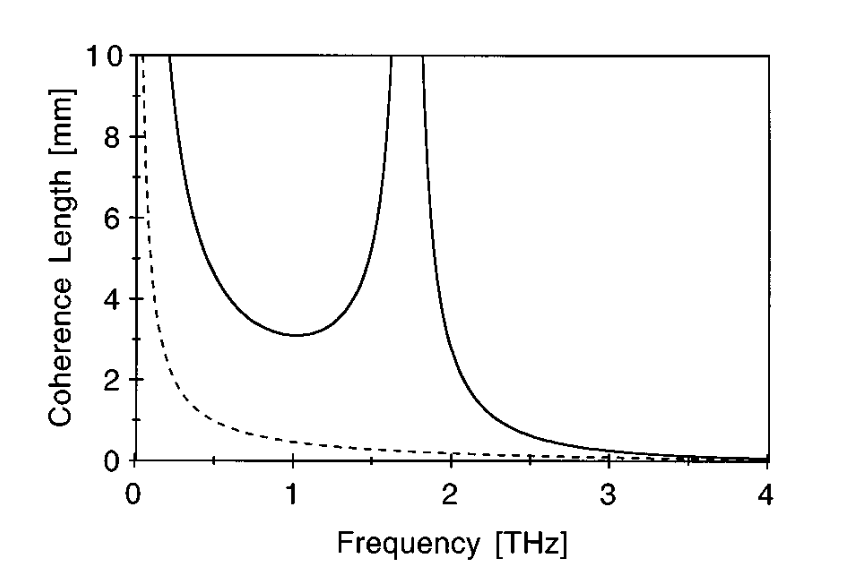
\includegraphics[width=0.5\textwidth]{refferenced_pic/coherence_length_ZnTe.png}
    \caption{The coherence length of a $\SI{800}{\nano\meter}$ laser pulse and $\si{\tera\hertz}$ radiation in dependence on the $\si{\tera\hertz}$ frequency.
    The solid line includes the effect of dispersion at optical frequencies. The dotted line neglects the dispersion at optical frequencies \cite{coherence_legnth}.}
    \label{fig:coherence_legnth}
\end{figure}
\textbf{Platzhalter für Grafik mit kohärenzlänge von GaP falls ich dazu was finde}
% I need a paper to refernce the coherence length of GaP
\FloatBarrier
